\documentclass[a4paper, 11pt]{article}

\usepackage[utf8]{inputenc}
\usepackage[T1]{fontenc}
\usepackage[francais]{babel}

\usepackage{graphicx}
\usepackage{float}
\usepackage{listings}
\newcommand{\HRule}{\rule{\linewidth}{0.5mm}}

\title{Projet tutoré\\Simulation de pliage dans un outillage progressif}
\author{Ariane LEFEBVRE \and Pablo COVES}
\date{}

\begin{document}
\begin{titlepage}
    \begin{center}
        
\includegraphics[width=0.23\textwidth]{img/imag.eps}~\\[1cm]
        \textsc{\LARGE Université Joseph FOURIER}\\[1.5cm]
        \textsc{\Large PROJET TUTORÉ}\\[0.5cm]
        \HRule \\[0.4cm]
        { \huge \bfseries Simulation de pliage dans un outillage progressif}\\[0.4cm]
        \HRule \\[1.5cm]
        \begin{minipage}{0.4\textwidth}
            \begin{flushleft} \large
                \emph{Auteurs:}\\
                Ariane LEFEBVRE\\
                Pablo COVES
            \end{flushleft}
        \end{minipage}
        \begin{minipage}{0.5\textwidth}
            \begin{flushright} \large
                \emph{Tuteurs:} \\
                M. Frédéric PONTAROLLO\\
                M. Christophe PICARD
            \end{flushright}
        \end{minipage}\\[2cm]
        
\includegraphics[width=.5\textwidth]{img/topSolid.eps}~\\[1cm]
        \vfill
        {\large \today}
    \end{center}
\end{titlepage}
\newpage
\tableofcontents
\newpage
\section{Notre projet}
\subsection{Le projet du client}
L'entreprise Missler Software  représentée par M. Frédéric PONTAROLLO travaillant au développement du logiciel TopSolid, nous a proposé le sujet suivant:
\begin{itemize}
        \renewcommand{\labelitemi}{$\bullet$}
    \item Implémenter une application permettant la simulation réaliste en deux dimensions du pliage d'une tôle par un outillage progressif.
La problématique étant d'approcher au mieux le comportement de la tôle lors du retour élastique ayant lieu durant le retrait du poinçon.
    \item Représenter l'aire couverte par le déplacement de la tôle, ainsi que la trajectoire d'un point choisi par l'utilisateur.
En effet les parties libres de la tôle lors de la déformation suivent une trajectoire non intuitive.
\end{itemize}

\subsection{Notre réécriture}
Nous devons créer une application prenant en entrée un fichier fourni par le client décrivant un état initial avant déformation ainsi que le déplacement du poinçon au cours du temps. Après discussion avec le client, nous considérons l'épaisseur de la tôle comme constante.\\
L'utilisateur doit pouvoir visualiser la simulation. Des interactions à la souris lui sont proposées afin de mesurer et suivre certains comportements relatifs à la déformation de la tôle.

\subsection{Tâches à réaliser}
Le groupe de projet était initialement composé de trois membres.
Deux issus de la spécialité Image et CAO ont étés attribués à la gestion de l'interface utilisateur, ainsi qu'au rendu graphique et du dialogue avec la partie simulation physique.
Cette dernière a été donnée à réaliser au troisième membre issu de la spécialité MCS.

\subsubsection{Interface utilisateur}
L'interface utilisateur consiste en une fenêtre permettant de choisir la durée d'une simulation ainsi que le pas temporel entre chaque étape de la déformation.
Elle est aussi dotée d'un lecteur donnant la possibilité à l'utilisateur de visualiser étape par étape ou sous forme d'une vidéo la déformation.\\
La zone de rendu implémentée en OpenGL est située à droite de la fenêtre, on y retrouve la scène composée de:
\begin{itemize}
        \renewcommand{\labelitemi}{$\bullet$}
    \item Une matrice, partie fixe sur laquelle va s'appuyer la tôle.
        Elle donne la forme finale de la tôle après déformation.
    \item Un dévêtisseur, partie mobile qui vient fixer la tôle sur la matrice.
        Il garantit l'immobilité de certains points de la tôle au cours de tout le procédé de pliage.
    \item Un poinçon, partie mobile qui vient frapper la tôle jusqu'à déformation complète de la matière, puis revient en position initiale.
    \item La tôle, la seule partie déformable de la scène.
        Elle est fixée entre la matrice et le dévêtisseur.
        Durant la simulation elle subit des forces associées au poinçon et à la matrice qui lui donneront sa forme finale.
    \item La fibre neutre, partie de la tôle sur laquelle ne s'applique aucune compression ou extension, lors de la déformation.
        Sa longueur reste fixe au cours du temps.
\end{itemize}
L'utilisateur est en mesure d'afficher l'aire couverte par le déplacement de la tôle au cours de la déformation.
Deux interactions à la souris sont offertes à l'utilisateur.
La première permet de suivre la trajectoire d'un point de la tôle.
La deuxième affiche la distance entre deux points préalablement sélectionnés.

\subsubsection{Chargement d'une scène}
Une scène est décrite par un fichier au format XML (Exemple en Annexe 1) contenant les différentes informations permettant la réalisation de la simulation d'une déformation.
Un parseur est donc nécessaire afin de remplir les différentes structures de données qui serviront aux calculs et au rendu.

\subsubsection{Moteur de déformation par éléments finis}
La partie du projet concernant la déformation à proprement parler devait être réalisée par notre trinôme de la spécialité MCS.
Elle a été remplacée par M.
Christophe Picard notre tuteur enseignant.
De ce fait et ne connaissant pas les détails de l'implémentation, nous considérerons cette partie comme une boîte noire dans la suite de ce rapport.\\
Un dialogue doit être implémenté pour envoyer les informations nécessaires à la déformation ainsi que récupérer les résultats de chaque étape.

\subsection{Les livrables en fin de projet}
Nous avons répondu à ce jour aux spécifications concernant la partie Image et CAO.
Seule manque la communication entre le moteur de déformation et l'application.\\
Il est possible de visualiser l'intégralité de la simulation grâce au lecteur, qui permet également de choisir une étape en particulier.\\
Les deux interactions à la souris sont accessibles, ainsi que l'affichage de l'aire couverte par la tôle au cours du temps.\\
L'intégralité du code produit et sa documentation seront mis à la disposition du client.

\section{Description des données disponibles}
Le client nous fournit le fichier XML correspondant à la scène qu'il souhaite simuler.
Nous avons précisé au client la structure du document correspondant à notre parseur.\\
Les informations contenues sont:
\begin{itemize}
        \renewcommand{\labelitemi}{$\bullet$}
    \item Un polygone définissant la matrice.
    \item Un polygone décrivant le dévêtisseur.
    \item Deux polygones définissant les positions haute et basse du poinçon.
        Il nous appartient de lui donner un déplacement réaliste.
    \item La tôle décrite par son épaisseur, un polygone définissant son contour ainsi qu'une courbe précisant l'emplacement de la fibre neutre.
\end{itemize}

\section{Description des méthodes}
\subsection{Introduction à la méthodologie générale}
Nous avons décidé d'utiliser un Model View Controler (MVC) qui correspond à la répartition des tâches entre les membres du groupe.\\
L'un s'est chargé de développer un prototype d'interface graphique afin de tester les premières implémentations.
Durant ce temps l'autre avait pour tâche la mise en place des structures de données et le parseur permettant leur instanciation.\\
Nous avons ensuite œuvré en parallèle sur le rendu: l'un sur le modèle et l'autre sur la vue.

\subsection{Méthodes utilisées ou envisagées}
\subsubsection{Déplacement du poinçon}
Le déplacement du poinçon est réalisé par un système de bielle manivelle dont nous avons établi la position du poinçon par rapport au temps dont voici l'équation:\\
\begin{center}
    $P(t) = \frac{-Dmax}{2}*\cos(\frac{2}{Tmax}*\pi*t)+\frac{Dmax}{2}$
\end{center}

\subsubsection{Interactions à la souris}
Lors des interactions souris par l'utilisateur, il nous a été nécessaire de retrouver les coordonnées du point OpenGL par rapport au point cliqué car la scène affichée a pu être modifiée par zooms et/ou translations.

\subsubsection{Affichage de formes complexes}
Dans le cadre de scènes comportant des objets de forme concave, il est nécessaire de les trianguler pour effectuer ensuite l'affichage correct par OpenGL.
Nous avons tenté d'effectuer cette triangulation, mais comme nous ne savions pas comment allaient être formés les objets renvoyés par le moteur de déformation, nous avons interrompu cette implémentation.

\subsection{Procédés de validation}
Étant donné que nous travaillions sur le rendu dans l'interface graphique, nous pouvions facilement visualiser le résultat.
Nous avons donc réalisé des tests unitaires suite à l'implémentation de chaque fonction.

\section{Résultats}
Nous n'avons pas eu de retour du moteur de déformation à l'heure actuelle.
Les images présentées dans cette partie sont issues d'une simulation naïve d'une déformation simple.

\subsection{Expérimentations réalisées}
\subsubsection{Simulation simple}
Dans cette simulation, la tôle représentée en vert avec sa fibre neutre en noir est maintenue à gauche entre la matrice en rouge et le dévêtisseur en jaune.
Le poinçon en bleu descend à la verticale, pour venir frapper la tôle.
\begin{figure}[H]
    \begin{center}
        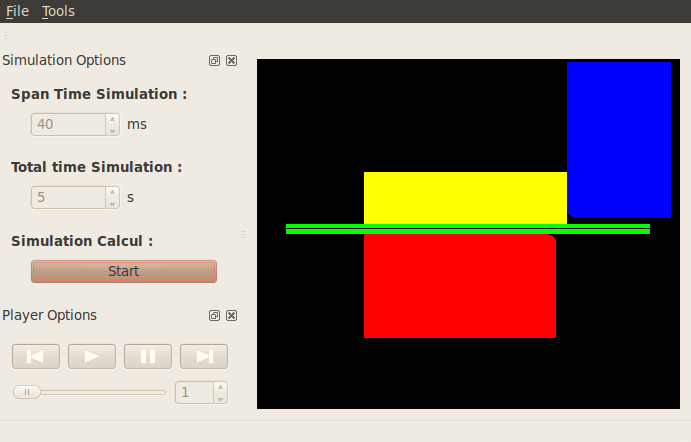
\includegraphics[width=.8\textwidth]{img/fenetreInitiale.png}
    \end{center}
    \caption{Scène avant déformation}
\end{figure}
\begin{figure}[H]
    \begin{center}
        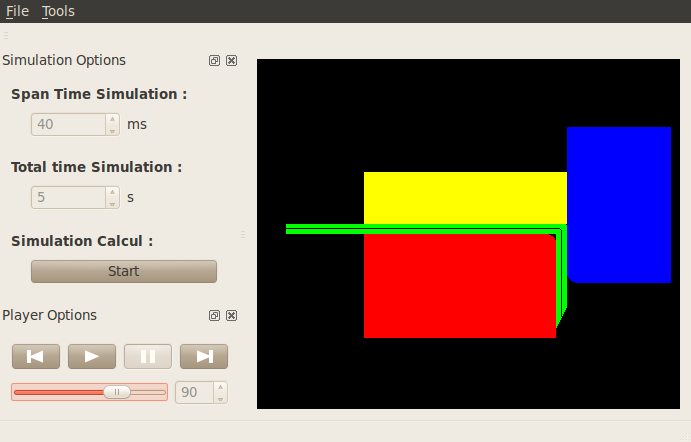
\includegraphics[width=.8\textwidth]{img/fenetreInitiale2.png}
    \end{center}
    \caption{Scène après déformation}
\end{figure}

\subsubsection{Suivi d'un point}
L'image suivante met en évidence la trajectoire d'un point de la tôle au cours de la simulation.
Le point à suivre correspond au point de la tôle le plus proche du curseur lors du clic à la souris.
Les coordonnées de ce point sont précisées dans la barre de statut en bas à gauche de la fenêtre.
\begin{figure}[H]
    \begin{center}
        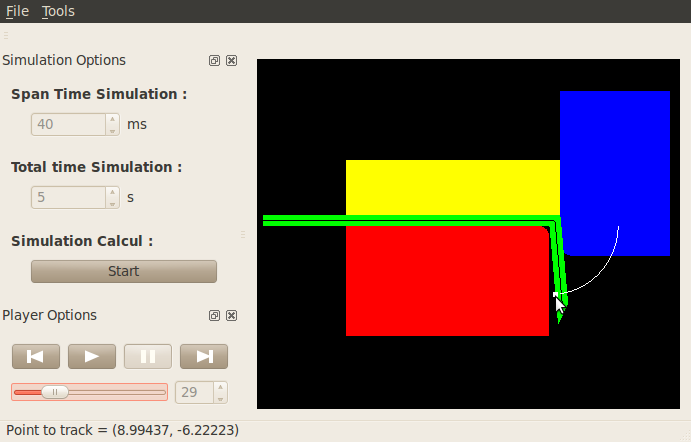
\includegraphics[width=.8\textwidth]{img/tracking.png}
    \end{center}
    \caption{Trajectoire d'un point choisi}
\end{figure}

\subsubsection{Distance entre deux points}
À partir de deux points sélectionnés par l'utilisateur, la distance réelle en millimètre est calculée puis affichée dans la barre de statut.
\begin{figure}[H]
    \begin{center}
        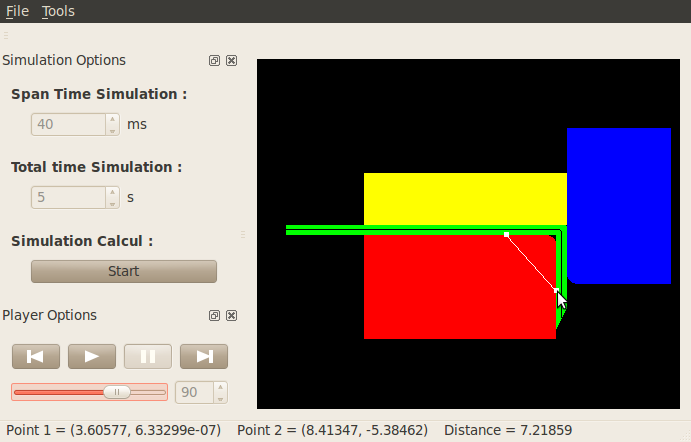
\includegraphics[width=.8\textwidth]{img/distance.png}
    \end{center}
    \caption{Distance entre deux points}
\end{figure}

\subsubsection{Aire couverte par la tôle}
Nous représentons en vert pâle l'aire couverte par la tôle au cours du temps.
\begin{figure}[H]
    \begin{center}
        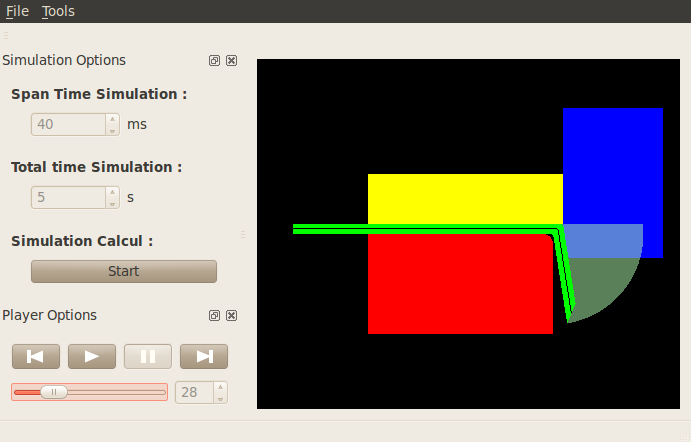
\includegraphics[width=.8\textwidth]{img/area.png}
    \end{center}
    \caption{Aire de couverture}
\end{figure}

\subsection{Évaluation de la qualité des résultats}
Les quatre spécifications principales étaient:
\begin{itemize}
        \renewcommand{\labelitemi}{$\bullet$}
    \item Le rendu d'une simulation de pliage en OpenGL.
        Nous avons un lecteur opérationnel, et robuste.
        Comme nous avons une simulation non réaliste dans l'attente des résultats du moteur de déformation, nous ne pouvons pas faire varier le pas et la durée totale de visualisation.\\
    \item Le suivi d'un point de la tôle au cours du temps.
        Nous affichons en blanc la trajectoire parcourue jusqu'à l'étape courante.
        L'utilisateur peut le modifier en cours de simulation et sa trajectoire est adaptée par rapport aux étapes précédentes en temps réel.
        Les coordonnées affichées sont les coordonnées du monde réel.\\
    \item Le calcul de distance entre deux points.
        Les deux points choisis sont affichés et reliés.
        Leurs coordonnées correspondent à celle dans le monde réel.
        Lorsque les deux points et la ligne sont affichés, s'il y a translation de la scène par l'utilisateur, cet affichage est perdu, mais les informations reste dans la barre de statut.\\
    \item L'affichage de l'aire couverte par la tôle au cours du temps.
        Nous affichons en vert pâle avec transparence l'aire de couverture jusqu'à l'étape courante.\\
\end{itemize}

\subsection{Critiques et commentaires}
Notre application remplie les spécifications initialement demandées par le client pour ce qui est des affichages et des interactions utilisateur.
Elle peut donc fonctionner sur une simulation réaliste.
Cependant, en l'absence de la boîte noire qu'est le moteur de déformation, nous avons dû créer notre propre simulation, ce qui nous a amené à adapter le code initialement général pour ce cas particulier.\\
Nous avons fait face à plusieurs difficultés.
La prise en compte de formes complexes telles que des polygones concaves et/ou comportant des auto intersections afin de pouvoir les afficher correctement, nous ont pris de nombreuses heures sur ce projet.
Faute de temps nous avons été contraint d'abandonner cette implémentation.
Notre application ne peut donc pas afficher ces formes complexes correctement.\\
L'absence du troisième membre du groupe dès le début du projet a été un facteur limitant dans la compréhension et l'avancement général du projet.
Jusqu'à il y a deux semaines, nous ne savions pas comment palier à cette absence.\\

\section{Conclusion}
Pour conclure ce rapport, nous avons répondu aux spécifications du client sur la partie Image et CAO.
M. Frédéric PONTAROLLO et M. Christophe PICARD se sont rendus très disponibles et à notre écoute durant ce projet, nous les en remercions vivement.

\section{Diagramme de Gantt}
\subsection{Diagramme de Gantt initialement prévu au début du projet}
\begin{figure}[H]
    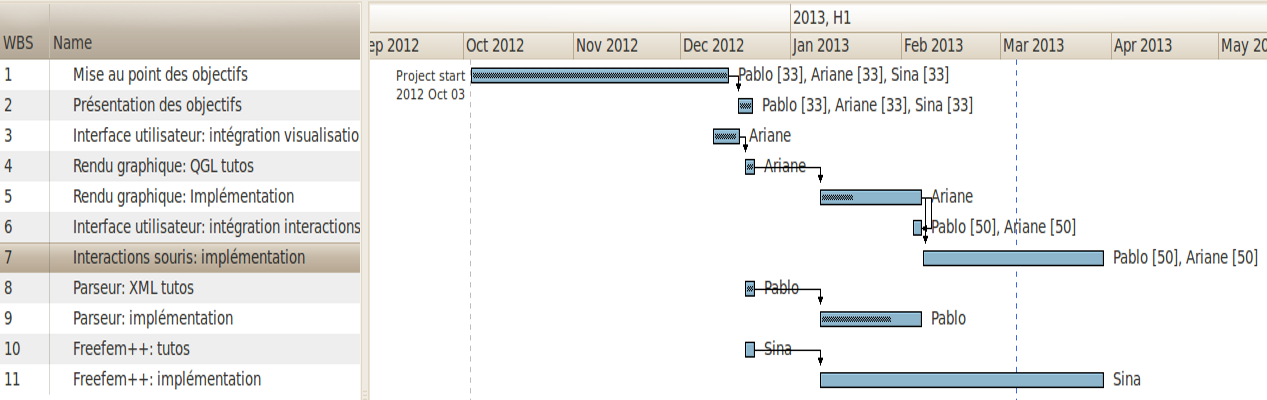
\includegraphics[width=\textwidth]{img/gantt.png}
    \caption{Gantt: début de projet}
\end{figure}
\subsection{Diagramme de Gantt revu et corrigé}
\begin{figure}[H]
    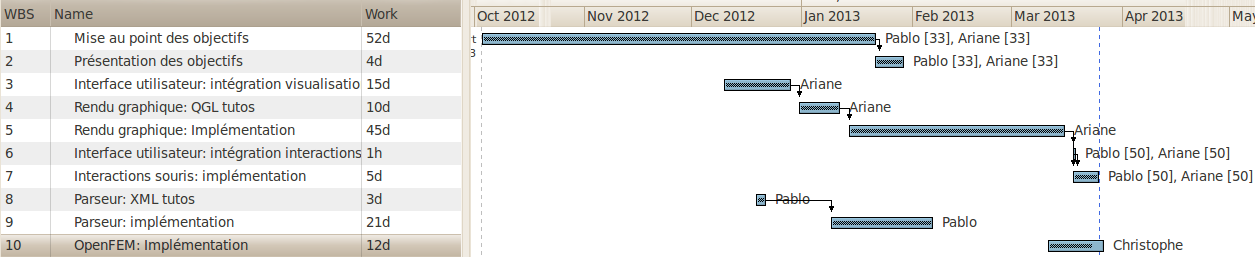
\includegraphics[width=\textwidth]{img/GanttFin.png}
    \caption{Gantt: fin de projet}
\end{figure}

\listoffigures 

\newpage
\appendix
\section{Fichier de scène au format XML}
\begin{lstlisting}[language=xml]
<scene>
<matrix>
<point x="7.45" y="0.00"/>
<point x="-10.00" y="0.00"/>
<point x="-10.00" y="-10.00"/>
<point x="8.45" y="-10.00"/>
<point x="8.45" y="-1.00"/>
<point x="8.45" y="-0.92"/>
<point x="8.44" y="-0.84"/>
<point x="8.43" y="-0.77"/>
<point x="8.40" y="-0.69"/>
<point x="8.38" y="-0.62"/>
<point x="8.34" y="-0.55"/>
<point x="8.31" y="-0.48"/>
<point x="8.26" y="-0.41"/>
<point x="8.21" y="-0.35"/>
<point x="8.16" y="-0.29"/>
<point x="8.10" y="-0.24"/>
<point x="8.04" y="-0.19"/>
<point x="7.98" y="-0.15"/>
<point x="7.91" y="-0.11"/>
<point x="7.84" y="-0.08"/>
<point x="7.76" y="-0.05"/>
<point x="7.69" y="-0.03"/>
<point x="7.61" y="-0.01"/>
<point x="7.53" y="-0.00"/>
</matrix>
<strippers>
<stripper>
<up>
<point x="9.45" y="6.00"/>
<point x="-10.00" y="6.00"/>
<point x="-10.00" y="1.00"/>
<point x="9.45" y="1.00"/>
</up>
<down>
<point x="9.45" y="6.00"/>
<point x="-10.00" y="6.00"/>
<point x="-10.00" y="1.00"/>
<point x="9.45" y="1.00"/>
</down>
</stripper>
</strippers>
<punch>
<up>
<point x="19.45" y="1.50"/>
<point x="19.45" y="16.50"/>
<point x="9.45" y="16.50"/>
<point x="9.45" y="2.50"/>
<point x="9.46" y="2.42"/>
<point x="9.47" y="2.34"/>
<point x="9.48" y="2.27"/>
<point x="9.50" y="2.19"/>
<point x="9.53" y="2.12"/>
<point x="9.56" y="2.05"/>
<point x="9.60" y="1.98"/>
<point x="9.64" y="1.91"/>
<point x="9.69" y="1.85"/>
<point x="9.75" y="1.79"/>
<point x="9.80" y="1.74"/>
<point x="9.87" y="1.69"/>
<point x="9.93" y="1.65"/>
<point x="10.00" y="1.61"/>
<point x="10.07" y="1.58"/>
<point x="10.14" y="1.55"/>
<point x="10.22" y="1.53"/>
<point x="10.30" y="1.51"/>
<point x="10.37" y="1.50"/>
<point x="10.45" y="1.50"/>
</up>
<down>
<point x="19.45" y="1.50"/>
<point x="19.45" y="16.50"/>
<point x="9.45" y="16.50"/>
<point x="9.45" y="2.50"/>
<point x="9.46" y="2.42"/>
<point x="9.47" y="2.34"/>
<point x="9.48" y="2.27"/>
<point x="9.50" y="2.19"/>
<point x="9.53" y="2.12"/>
<point x="9.56" y="2.05"/>
<point x="9.60" y="1.98"/>
<point x="9.64" y="1.91"/>
<point x="9.69" y="1.85"/>
<point x="9.75" y="1.79"/>
<point x="9.80" y="1.74"/>
<point x="9.87" y="1.69"/>
<point x="9.93" y="1.65"/>
<point x="10.00" y="1.61"/>
<point x="10.07" y="1.58"/>
<point x="10.14" y="1.55"/>
<point x="10.22" y="1.53"/>
<point x="10.30" y="1.51"/>
<point x="10.37" y="1.50"/>
<point x="10.45" y="1.50"/>
</down>
</punch>
<sheet thickness="1">
<geometry>
<point x="-17.55" y="1.00"/>
<point x="-17.55" y="0.00"/>
<point x="17.50" y="0.00"/>
<point x="17.50" y="1.00"/>
</geometry>
<neutral>
<point x="-17.55" y="0.50"/>
<point x="17.50" y="0.50"/>
</neutral>
</sheet>
</scene>
\end{lstlisting}
\end{document}
